\graphicspath{{main/chapter1/Intro: structural repeat/figs/}}
\section{Repetition as an experience}
\begin{comment}
Section goal: Motivate the notion of structural repeat
- [requirement 1] This section should be readable for general audience. All examples should be simple, intuitive, and common. 
- [requirement 2] This section should fully establish why defining repeat as a cognitive phenomenon is nontrivial. 
- [requirement 3] This section should build up the concept (structural repeats) incrementally, starting from the simplest notion of repeat. Each increment of the concept should highlight the part that is new and explain what additional explanation power it gives. 
- [requirement 4] This section should only introduce the formal notations only after the reader has understood the nuances of the concept intuitively and verbally. 

Plan: 
    - intro
    - First approximation: Equality of the observations 
        - Can explain: 
        - Can't explain: Postman example of ``doing the same thing''
        - Limitation: we sometimes also experience non-exact repeat
        - Core problem: (Categorization) An entity is characterized by its external properties and affordance.  
    - Second approximation: Equality of the Abstraction 
        - e.g. conceptual category, intention, particular features, internal relations
         (the instantiation of a abstract concept can be subsumed as a generative program)

        - Can't distinguish: parralel syntax 
    - Third approximation: Equality of the Interpretation 
        - Equality of the generative program underlying the observation.

    - Structural repeat




    
    Extensional vs Intentional equality
    - Third approximation: Intentional equality of the generative programs underlying the observation
    https://oecs.mit.edu/pub/vgigt1aq/release/1?from=10215&to=11248
    https://oecs.mit.edu/pub/vgigt1aq/release/1?from=12735&to=13964

   "By viewing causal induction as the result of domain-general
    statistical inference guided by domain-specific causal theories, our
    framework provides a unified account of a set of phenomena that
    have traditionally been viewed as distinct." (Griffiths Tenenbaum, 2009,Theory-Based Causal Induction)
\end{comment}

% The central topic of this thesis is about the computational modeling of repetitions in music in a cognitively plausible way. 
% Although repetition in music might be different from other domains, we first focus on the aspects that is generally applicable in other domains. 
% Repetition is a core feature of our musical experience. Since music is fundamentally a mental phenomenon, perhaps it is helpful to first take a birds-eye-view on how human we experience repetition in general.

We experience repetition in diverse domains: we discern shared narrative structures across novels, films, and music, and we uncover universal laws governing phenomena as distinct as ocean currents and atmospheric dynamics. Moreover, humans can abstract patterns of patterns, as seen in the application of category theory to mathematics and programming. These examples illustrate our remarkable ability to not only detect abstract repetitions but also to productively employ them in navigating both the physical and mental worlds.

Repeat, as we intuitively perceive it, is surprisingly nontrivial to formalize. As the term ``repeat'' is overloaded with multiple interpretations, we begin this section by clarify the  \emph{object} of repeat. 

\subsection{Repeated observations}
Perhaps our simplest and most direct experience of repeat comes from the repetition of concrete observations. ``Observation'' refers to all kinds of direct sensory input. For instance, an ongoing fire siren corresponds to a repeat of a specific sound across time. The decorative motifs found in mosaic tiling are repeats of a visual symbol across space. The periodic motion of a pendulum contains repeats of a specific movement.

% \begin{figure}
%     \centering 
%     
\includegraphics[width=0.3\linewidth]{Venetian floor.png}
%     \caption{}
%     \label{}
% \end{figure}


To put it formally: 
\begin{equation} 
    \tag{Approximation 1}
    \llbracket x_2 \ \emph{repeats}\  x_1  \rrbracket\footnote{We adopt the notation $\llbracket \dots \rrbracket$ from formal semantics as a function that maps a expression to its truth condition}  =\left\{ x_2 = x_1\right\}
    \label{eq: approximation 1}
\end{equation}
Our first definition is simple and precise, and its mental processing of can be computationally modelled as pattern identification/matching.

However, exact pattern matching does not cover many of our usual experience of repeat. Consider a postman, when frustrated by his mundane work, complains about ``doing the same thing'' over and over again. Clearly, by ``doing the same thing,'' our imaginary postman does not mean it as repeating a list of concrete physical actions (e.g., turning right on the crossroad at 7:23 am, and stopping his car at the exact same spot). If the postman's job can be just explained as such, imagine the catastrophes caused by a mail robot programmed to do exactly that. 

In order to make the postman's expression work, our model of repeat should allow some degrees of flexibility. For example, there are multiple ways to achieve the same task of ``parking the car'' depending on the situation at hand. What if the closest parking slot is occupied? What if there are kids walking by? What if there are construction works blocking the entire side of the street? ``Just do the sensible things'' would be a typical response from humans. In those scenarios, the observed actions would be adapted to include extra stepping on gas and break, checking the mirrors/traffic lights/pedestrians, looking for available parking slots. Then to our robot friend, in what ground can it understand these ``sensible adaptions'' of actions as being the ``same''? 

If we understand repeat based on the properties of the observations themselves, one way to extend our first approximation is to replace the equality in \ref{eq: approximation 1} by a  similarity function. For example, one might say if two list of actions both ends with stopping the car and getting out the car, we define a high similarity among them. 




\subsection{Repeated abstractions}

There are cases where our experience of repeat is not about the similarity of the observations at all. Imagine the cityscape of New York where we find repetitions of buildings. Each building can be very different from the image perspective. Base on the visual features alone, one might say the World Trade Center Transportation Hub (Figure \ref{fig: Oculus}) is closer to a dove than a building,\footnote{The architect Santiago Calatrava use the appearance of a dove as a symbol for peace.} which is entirely valid as an \emph{artistic} interpretation. However, few people would actually believe it is a real dove and would more likely to see it as a building in a shape of a dove. 

\begin{figure} 
    \centering 
    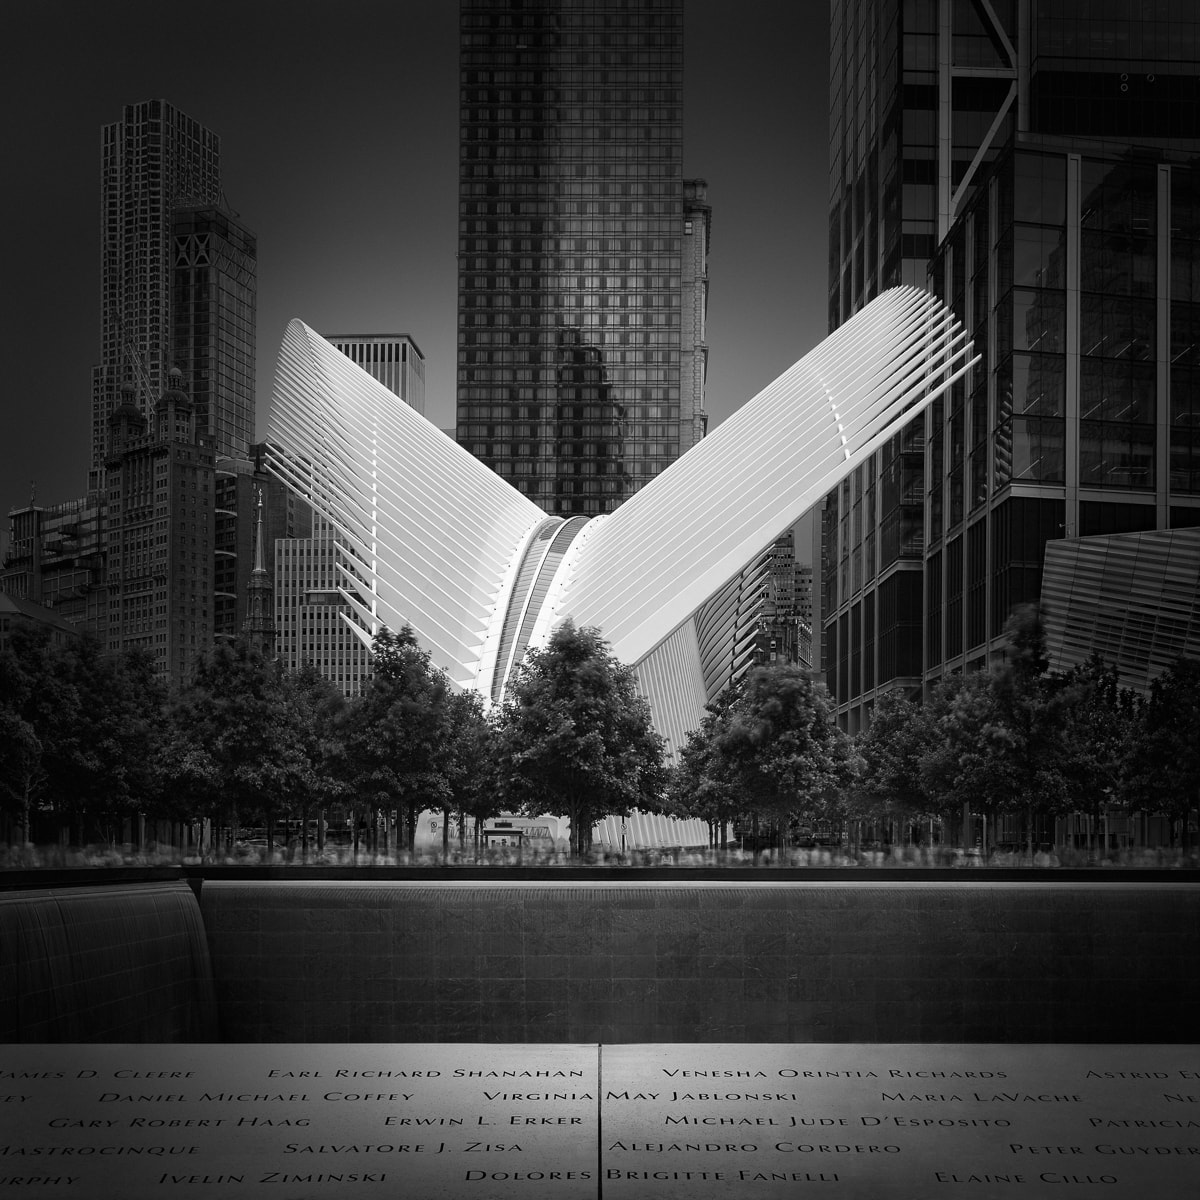
\includegraphics[width=0.5\linewidth]{Julia-Anna-Gospodarou_Flying-Away_-New-York-Oculus-Memorial-Pools_1200px.jpg}
    \caption{Flying Away I -- Oculus by Calatrava New York. The photograph was shot in New York and was first published in August 2019.}
    \label{fig: Oculus}
\end{figure}
The reason we perceive repeat in this circumstance is that we interpret these visuals as concrete instances of the same abstract concept---building---which we know its characterizing properties and functions. Thus, the core problem of the first definition is that it describes the phenomenon of the perceived repeat purely as a property of the observations themselves, without involving a mental understanding of the observations. 

% If we go back to visual patterns, we find variations also across instances of repeats. So our "ill-defined" notion of repeat also fails there. So the problem of our definition is just limited to one domain but is a general issue.
% For visual case, one can potentially measure the pixel-wise L2 distance (MSE). 





If we think of ``mental understanding'' as the ability to associate a specific token with its category/type, our next approximation of repeat would be ``instantiations of the same category/type.'' 
\begin{equation} 
    \tag{Approximation 2}
    \llbracket x_2 \ \emph{repeats}\  x_1  \rrbracket = \left\{ \text{Type}(x_1) = \text{Type}(x_2)\right\}
\end{equation}

Categorization refers to the mental process of forming a system of tokens (observations) and their types/category (abstractions) and is considered a fundemetal human cognitive capacity.\cite{}
Computational mechanisms of human categorization has been theorized with varying representations of conceptual category. One idea is to use a ``typical'' observation as the representation of a conceptual category. One prominent cognitive theory that resembles such an idea is \emph{Prototype theory}\cite{} developed by psychologist Eleanor Rosch. Prototype theory describe the cognitive process of categorization as measuing the similarity between the observation with an ideal prototype of a concept in long term memory. In our postman example, it entails that we compare a specific realization of the action ``parking the car'' to a prototypical notion of parking the car in our memory (the prototype might differ from person to person). This can explain the postman's notion of ``doing the same thing'' by considering the specific implemetations of the actions as similar to an ideal version of it. It is worth noting that the ideal prototype may not actually exist in reality. For example a perfect circle does not exists in our physical world but it is still useful to categorize things base on ideal shapes. Continuing the same strand of thought, \emph{Exemplar theory}\cite{} propose that we do not just store one ideal prototype but all the instances of a concept, all of which may participate in the classification decision of an observation. These two notions of categorization manifests in data science as classification and clustering algorithms such as the Gaussian mixture model\cite{} and the k-nearest neighborhood\cite{}, which incorperates formal handling of the deviations from the representations (prototype or examplars) in memory. 


Another approach to categorization is based on traits or affordance of entities (e.g. being able to run and carry objects) rather than their observable attributes (e.g. having four wheels). In the postman's example, we can categorize concrete actions by their intended effect on the world, for example, ``inserting mail to mailbox'' can be represented as any action that result in mail being in the mailbox. Such external characterization forms a useful abstraction that enables greater generality both in classification and in production. It also aligns closer with humans intuition in cases of innovation (e.g. imagining the next generation of transportation).


By shifting the focus from observations to their mental abstractions, we can explain the postman's notion of ``doing the same thing'' as multiple instantiations of abstract action ``parking the car'' or ``inserting mail to mailbox'' on different situation-encoding parameters such as ``the location of the next closest parking slot'' and ``whether there are objects blocking the path''. In the case of New York's cityscape, each appearance of the buildings can be thought of as an instantiated token from the type ``building'' using different configurations such as the building's structure, style, material, as well as spatial attributes and lighting environment such as the angle facing the viewer, light source and shadows, etc. 


\begin{comment}reference: "Tenenbaum and Niyogi (2003) also
showed that people spontaneously organize objects into types on
the basis of their causal properties, forming abstract categories of
schematic blocks that cause one another to light up in a computer
simulation, and Kemp, Goodman, and Tenenbaum (2007) showed
that such categories could carry with them expectations about the
strength of causal relationships."
\end{comment}







\subsection{Repeated interpretations}

Despite the generality of the approach, it may sometimes ignore too much information that are critical for our experience of repeat. Let's reflect on the common expression "the history repeats itself", not as a historical and philosophical statement, but as a result of our perception of repeat. Certainly, the notion of repeat is not about a concrete chain of events (based on our first approximation); and arguably, not about the overall abstraction of the historical events (based on our second approximation). It is rather about the pattern of how the smaller abstracted events (e.g. improved education, war, enactment of certain kind of law) contributes to the more abstracted events (advancement in technology and innovation, economic crisis, social inequality) which in turn leading to bigger events (e.g. global competitiveness,) and ultimately to the most abstracted description (e.g. the rise and fall of civilizations). 

% \begin{figure}[]
%     \centering 
%     
\includegraphics[width=0.8\linewidth]{chinese peom surface}
%     \caption{Exerpts from the poem () written by Wang Wei (699–761 during Tang dynasty), translated by Xu Yuanchong}
%     % %Such kind of parallel is not an incident but almost a requirement in Tang poetry, which support human's ability the both recognize and generalize such patterns.}
%     \label{fig: Chinese poem surface}
% \end{figure}


% 
\begin{figure}
    \centering 
    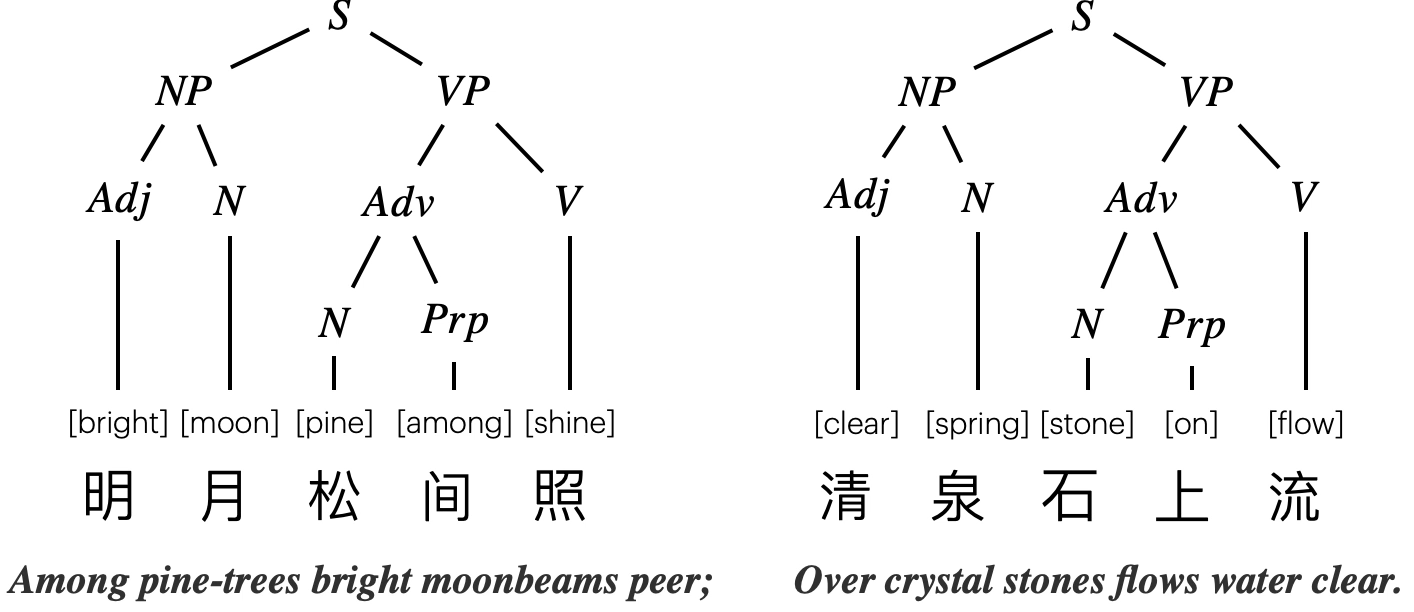
\includegraphics[width=0.8\linewidth]{Chinese poem.png}
    \caption{A poetry written by Wang Wei (699–761 during Tang dynasty), translated by Xu Yuanchong, exhibiting parallel syntactic structure.} 
    % %Such kind of parallel is not an incident but almost a requirement in Tang poetry, which support human's ability the both recognize and generalize such patterns.}
    \label{fig: Chinese poem}
\end{figure}


The same kind of inadequacy of our second approximation is revealed by an example of excerpt from a Chinese poem (Figure \ref{fig: Chinese poem}). One can notice that there are some correspondence between the structure of this two phrases. In terms of grouping, ``[bright] [moon]'' corresponds to ``[clear] [spring]'' and ``[pine] [among] [shine]'' corresponds to ``[stone] [on] [flow]''. Not only each of the corresponding character are from same syntactic category, the syntactic structures of the two phrases are identical as demonstrated in Figure \ref{fig: Chinese poem}. Furthermore, the meaning of the corresponding words all aims to convey a feeling of serenity. In fact, these associations that one of the stylistic criteria for Tang dynasty is the usage parallel construction. 
% 
Our percieved repeat (parallelism), even just on the syntactic level, can not be simply explained by that both phrases are noun phrases. If we substitute the second phrase with any other noun phrase, our previous experience of parallelism immediately disappear. If we explicitly factor in the interpretation about the observations, we are much closer to the kind of repeat shown in the Chinese poem example. Figure \ref{fig: Chinese poem} reveals the syntactic structure (as one kind of interpretation) underlies the two parallel phrases. 
% This two identical parse tree are the actually repeating object (in the strict sense).
Compares to our second approximation (which would summarize both phrases as noun phrases), the parse tree provide the extra process connecting the observation to the abstraction. It is via such identical connections we experience a sense of repeat.   

What is missing from our second approximation is the connection from the specific to the abstract. When describing repeat of this kind, we need to the able to refer to an underlying interpretation, a group of hierarchically organize relations linking layers abstractions to the concrete tokens. 

\begin{equation} 
    \tag{Approximation 3}
    \llbracket x_2 \ \emph{repeats}\  x_1  \rrbracket = \left\{ \exists R\ X_1 \ X_2 ,\quad  X_1 R x_1 \wedge   X_2 R x_2 \right\}
\end{equation}







% Perhaps a more general way to expressive our experience of repeat is \textbf{the reoccurrence of some invariance of interest underlying the observations}. 





% A natural next step of our approximation is: \textbf{outputs of the same program on given different inputs}. Here an important distinction is made: we test the equality of the programs instead of equality of their outputs. With this modification of our approximation, we can explain the postman's notion of ``doing the same thing'' as calling the same functions ``parking the car'' or ``inserting mail to mailboxes'' on different situation-encoding parameters such as ``the location of the next closest parking slot'' and ``whether there are objects blocking the path''. The output of these functions results in concrete actions, which are different on the face value. More precisely, if we have two observations $y_1$ and $y_2$, we say they are repeated if there exist a function $f$ and input parameters $x_1$ and $x_2$ such that $y_1 = f(x_1), y_2 = f(x_2)$.


% \begin{equation} 
%     \tag{Approximation 2}
%     \llbracket y_2 \ \emph{repeats}\  y_1  \rrbracket = \left\{ \exists f\ x_1\ x_2,\quad  f(x_1)=y_1 \wedge  f(x_2) = y_2\right\}
% \end{equation}






% One way to model such flexibility is to see these concrete instances of repeats as \textbf{outputs of the same program (model/function) but given different parameters}. This characterization is fairly simple to model computationally in the generative direction (e.g. as in procedurally generated visual scene), but is much harder the implement in the direction of perception.

% \begin{equation} 
%     \tag{}
%     \llbracket y_2 \ \emph{repeats}\  y_1  \rrbracket = \left\{ 
%         y_1=g(f_1(x_1)) \wedge y_2 = g(f_2(x_2))
%     \right\}
% \end{equation}


% \begin{table}
%     \centering
%     \begin{tabular}{p{0.3\linewidth}  c  c}
%         Approximations & Examples & Required mechanisms \\
%         \toprule
%         The same concrete observation occurs in different time and space.  & e & d\\
%         \hline
%         The same model being instantiated with different parameters. & df &\\
%         \hline
%         The same relation instantiated with different abstractions of observations. & df &
%     \end{tabular}
%     \caption{}
% \end{table}

% \begin{table}
%     \centering
%     \begin{tabular}{l l l}
%         Notion of equality & non-structural & structural \\
%         \toprule
%         Exact  & $\exists f g x_1 x_2, f(x_1) = g(x_2) \wedge f \simeq g$  & $\exists f g x_1 x_2, f(x_1) = g(x_2) \wedge f \equiv g$ 
%         % \hline
%         % Non-exact & $\exists f_1 f_2 g_1 g_2 x_1 x_2, f_1(f_2(x_1)) = g_1(g_2(x_2)) \wedge f_1 \simeq g_1$  & $\exists f_1 f_2 g_1 g_2 x_1 x_2, f_1(f_2(x_1)) = g_1(g_2(x_2)) \wedge f_1 \equiv g_1$ 

%     \end{tabular}
%     \caption{}
% \end{table}

% \begin{table}
%     \centering
%     \begin{tabular}{l p{0.3\linewidth} p{0.3\linewidth}}
%         $f$, $g$ share the same & upper-level & lower-level  \\
%         \toprule
%         formalization  & $\exists f_1 f_2 g_1 g_2, f = f_1 \circ f_2\wedge g = g_1 \circ g_2 \wedge f_1 \equiv g_1$  & $\exists f_1 f_2 g_1 g_2, f = f_1 \circ f_2\wedge g = g_1 \circ g_2 \wedge f_2 \equiv g_2$\\
%         \hline
%         examples & variations of K331 (same upper level reduction with different lower level realization) & bach C major prelude (same figuration across phrases with different harmony reduction)
%         % Non-exact & $\exists f_1 f_2 g_1 g_2 x_1 x_2, f_1(f_2(x_1)) = g_1(g_2(x_2)) \wedge f_1 \simeq g_1$  & $\exists f_1 f_2 g_1 g_2 x_1 x_2, f_1(f_2(x_1)) = g_1(g_2(x_2)) \wedge f_1 \equiv g_1$ 
%     \end{tabular}
%     \caption{}
% \end{table}




% \paragraph{Attempt 1: The same concrete observation occurs in different time and space.}

% Required computational mechanisms : 
%     - production: duplication 
%     - understanding: equality testing
% Failed reason: too little flexibility, does not take abstractions into account.

% \paragraph{Attempt 2: The same pattern being instantiated in different time and space.}

% Required Computational mechanisms (given the space of generative function) (on top of attempt 1): 
%     - production: sampling function parameters, function application
%     - understanding: 

% \paragraph{Attempt 3: The same groups of relation governing abstractions of observations.}




% \end{document}

\section{Structural Repeat}


Our experience of repeat can be enriched and deepened by structure. The previous three approximations for repetition captures increasingly nuanced experience of repeat via domain specific structure (see Table \ref{table: object of repeat}). In the first approximation, there is no structured knowledge or theory about the specific domain other than a notion of equality or similarity. In the second approximation, we assume an ontology of the domain that organize observations by their abstractions via a system of tokens and types. In the third approximation, we assume a casual theory which adds on top of the ontology, a set of primitive relations linking entities and their abstractions.\footnote{In particular, formal grammars can be seen as an instance of a causal theory where the ontology is the system of non-terminal and terminal symbols, and the primitive relations are the production rules.} 

\begin{table}
    \centering
    \begin{tabular}{l l}
        Object of repeat & Corresponding cognitive ability \\
        \toprule
        Concrete observations & Pattern matching\\
        Abstractions & Categorization\\
        Interpretations & Causal explanation

    \end{tabular}
    \caption{}
    \label{table: object of repeat}
\end{table}

In an informal way, ``structure'' describes ``how things can be put together'' or ``how things can be decomposed'' in a domain. When describing ``how things can be put together'', a good system would have a few rules but can explain potentially infinite combinations. To achieve this, one need to be able to describe combinations on the level of abstractions/types instead of the specific instances as it gives rise to the ability to generalize. In other words, one need an ontology of the domain.  

In natural language, words are abstracted into their \emph{syntactic categories}, whose valid combination is described by the \emph{syntax}. These two components specifies a causal theory of grammatically correct sentences.

In action planning, actions are abstracted into their \emph{intended goals}, whose valid combination is described by the \emph{inferences rules in logic}. These two components specifies a causal theory of goal-oriented actions. 

In music, concrete notes are abstracted into \emph{harmonies and voices or tones},\footnote{Notes without temporal attributes} whose valid combination is described by rules of \emph{tonal structure}. These two component specifies a causal theory of tonal polyphony.

The main theme of this thesis is to understand repetition respecting the underlying causal structure. To be able to computationally model causal theory in a way that is domain general, we need to adopt a uniform representation of a causal theory. Let us examine three examples. 


\begin{comment} These three components are an ontology, a set of principles that
identify plausible relations, and a statement of the functional form
of those relations.
\end{comment}

\begin{comment}
    principles and implementation of deductive parsing "The increased expressive power
    of adjunction allows important natural-language phenomena such as long-distance
    dependencies to be expressed locally in the grammar, that is, within the relevant
    lexical entries, rather than by many specialized context-free rules [14]."
\end{comment}


\subsection{A causal structure of Chinese poetry}

In this example, the real observable entities are the words ``[bright]'',``[moon]'', etc. The job of the causal theory is to explain the occurrence of these specific sequence words. The Chinese grammar fulfills the role of a causal theory in the following way. First an ontology of the entities (words) are specified in two parts: (1) the space of types, represented by syntactic categories such as nouns, verb, etc, and (2) the association from tokens to types\footnote{This corresponds to non-terminal symbols and termination rules in formal grammar}. Second a finite list of relations associating a type with $n$ tokens or types, encoding how each syntactic category could be elaborated into multiple categories\footnote{These relations corresponds to a subset of the production rules in formall grammar where the right-hand side does not contain non-terminals.}. For example, the relation $R1$ says that a sentence and be constructed as a noun phrase followed by a verb phrase, which asserts the grammatical validity of combining ``[bright] [moon]'' with ``[pine] [among] [shine]''\footnote{The second part is valid according to the Chinese grammar and is invalid with the English grammar.}.

\newcommand{\poetryToken}{
    \begin{minipage}{0.3\linewidth}
    \begin{align*}
    \text{bright, clear}\\
    \text{moon, pine, spring, stone}\\
    \text{among, on}\\
    \text{shine, flow}
    \end{align*}
    \end{minipage}
}

\newcommand{\poetryType}{
    {\begin{minipage}{0.1\linewidth}\centering 
        $S$\\
        $NP$ \\ 
        $N$ \\ 
        $Adj$ \\ 
        $Adv$ \\ 
        $Prp$
        \end{minipage}}
}

\newcommand{\hRelation}[3]{$\displaystyle \frac{#2}{#3}{#1}$}
% \newcommand{\hRelation}[3]{$\displaystyle {\small \text{#2}}\xrightarrow{#1}{\small \text{#3}}$}

\newcommand{\poetryRelation}{
    \begin{tabular}{lll}
        \hRelation{\textsc{R}_1}{S}{NP \quad VP} &
        \hRelation{\textsc{R}_2}{NP}{Adj \quad N}&
        \hRelation{\textsc{R}_3}{VP}{Adv \quad V}
        \\
        \hRelation{\textsc{R}_4}{Adv}{N \quad Prp}&
        \multicolumn{2}{l}{\hRelation{\textsc{Term}_N}{N}{\color{gray}\text{moom | pine | spring | stone}}}
        \\
        \hRelation{\textsc{Term}_{Adj}}{Adj}{\color{gray}\text{bright | clear}}&
        \hRelation{\textsc{Term}_{Prp}}{Prp}{\color{gray}\text{among | on}}&
        \hRelation{\textsc{Term}_{V}}{V}{\color{gray}\text{shine | flow}}
    \end{tabular}
}



\begin{table}[h]
    \centering
    \bgroup
    \renewcommand{\arraystretch}{4}
    \begin{tabular}{c|cc}
        \toprule
        \textbf{Ontology} & 
        $\text{types} = \left\{\poetryType\right\}$
        &
        $\text{tokens} = \left\{{\poetryToken}\right\}$
        \\
        \hline
        
        \textbf{Relations} & 
            \multicolumn{2}{c}{
                \poetryRelation
            }
        \\
        \bottomrule
    \end{tabular}
    \egroup
    \caption{A simplified casual theory in the domain of language (the Chinese poem example)}
\end{table}



\newcommand{\Term}{\textsc{Term}}
\begin{figure}[h]
    \centering 
    \begin{tikzpicture}[
        % every tree node/.style={draw,circle},
        level distance=1cm,sibling distance=0.3cm,
        edge from parent path={(\tikzparentnode) -- (\tikzchildnode)},
        % every edge/.append style={color=red}
        ],
        % \tikzset{level 2+/.style={color=orange}}
        \Tree 
            [.(;)
                [.$\color{orange}\textsc{R}_1$ 
                \edge [color=orange] node[auto=right, font=\tiny] {NP};
                    [.$\color{orange}\textsc{R}_2$ 
                        \edge[color=orange] node[auto=right, font=\tiny] {Adj};$\color{orange}\Term$  
                        \edge[color=orange] node[auto=left, font=\tiny] {N};$\color{orange}\Term$ 
                    ] 
                \edge[color=orange] node[auto=left, font=\tiny] {VP};
                    [.$\color{orange}\textsc{R}_3$ 
                        \edge[color=orange] node[auto=right, font=\tiny] {Adv};
                        [.$\color{orange}\textsc{R}_4$ 
                        \edge[color=orange] node[auto=right, font=\tiny] {N};$\color{orange}\Term$ 
                        \edge[color=orange] node[auto=left, font=\tiny] {Prp}; $\color{orange}\Term$
                        ] 
                        \edge[color=orange] node[auto=left, font=\tiny] {V}; $\color{orange}\Term$
                    ] 
                ]
                [.$\color{orange}\textsc{R}_1$ 
                \edge[color=orange] node[auto=right, font=\tiny] {NP};
                    [.$\color{orange}\textsc{R}_2$ 
                        \edge[color=orange] node[auto=right, font=\tiny] {Adj};$\color{orange}\Term$  
                        \edge[color=orange] node[auto=left, font=\tiny] {N};$\color{orange}\Term$ 
                    ] 
                \edge[color=orange] node[auto=left, font=\tiny] {VP};
                    [.$\color{orange}\textsc{R}_3$ 
                        \edge[color=orange] node[auto=right, font=\tiny] {Adv};
                        [.$\color{orange}\textsc{R}_4$ 
                        \edge[color=orange] node[auto=right, font=\tiny] {N};$\color{orange}\Term$ 
                        \edge[color=orange] node[auto=left, font=\tiny] {Prp}; $\color{orange}\Term$
                        ] 
                        \edge[color=orange] node[auto=left, font=\tiny] {V}; $\color{orange}\Term$
                    ] 
                ] 
            ]
    \end{tikzpicture}
    \caption{The composition of domain specific relations as repeated object in the Chinese poetry example}
    \label{fig: relation tree (poetry)}
\end{figure}

With a causal theory in place, a causal explanation is made concrete as a composition of the domain specific relations (Figure. \ref{fig: relation tree (poetry)}), representing an interpretation of the observations. At this point one might wonder why we do not use a tree use node are types (as the ones in Figure \ref{fig: Chinese poem}). The answer is that when the relations have multiple instantiations (if it involves variables for instance), a tree of types could not capture the sameness of the underlying relation. However, a tree whose node are relation explicitly represents the structure of the interpretation. If we understand the composition of relations as a generative program, then the type tree corresponds to the input and output of our program after each function call, whereas the relation tree corresponds to the program itself. Our next example in action planning demonstrates the additional expressive power of relation tree when a relation have multiple instantiations.
% Parallel syntax is the phenomenon when two phrases have the identical syntactic structure. An example is shown in Figure \ref{fig: Chinese poem}. This kind of repeat is hardly a happy coincidence. It is often the case that the semantic meanings also forms either synonyms or contrast. 

\subsection{A causal structure of action planning for making coffee}
Imagine John performed the following list of actions: he measures 18 grams of coffee ground, put these measured coffee ground into a coffee maker, he then measures 150 ml of water, and put the measured water into the coffee maker, then he activates the coffee machine. We are first interested in how we can understand John's action as a coherent realization of a goal, which is answered by a causal theory of the domain. We further ask how can be capture our percieved repeat within this list of actions, which is answered by infering the shared component within a causal explaination of the actions. 

% We can perceive the repetition of this composite actions "measuring x amount of y and put y into the coffee maker". 
% The ontology of action answers two questions: what does each action achieve and how does these list of actions accomplish a single goal? 
Similar to the Chinese poem example, the ontology of action can be defined in two parts (1) a space of types represent goals and (2) a mapping from tokens to types representing how an action can be understood as to achieve a goal. To make things simple, goals are interpreted as changes in the state of the world, denoted by an arrow from state before the action to the  state after the action. For example, the overarching goal in this example is that John want to transform his state from "having coffee bean and water supply" into ``having a cup of coffee''.

Goals can be combined in two general and natural ways, the first is sequential composition (chaining): if we know how to accomplish $x\to z$ and $z\to y$ we can accomplish the goal $x \to y$ by concatenating the two actions (also feeding the result of the action to the next action). The second is parallel composition, if we can accomplish $x_1 \to y_1$ and $x_2 \to y_2$, we can also accomplish $(x_1,x_2) \to (y_1,y_2)$. The tuple notation denotes the conjunction of states. 

These rules about how goal can be decomposed forms the space of relations in our action planning domain.

\newcommand{\actionType}{
    \begin{minipage}{0.6\linewidth}
        {\begin{align*}
        \text{types} &= \{ \text{$s_1 \to s_2$ | $s_1,s_2 \in \text{WorldState}$} \}\\
        \text{WorldState} &= \{\text{Having $q$ | $q \in$ Quantified} \} \\
        &\cup \{\text{$x$ in machine | $x\in$ Quantified\}}\\
        &\cup \text{WorldState $\times$ WorldState}\\
        \text{Quantified} &= \{\text{$x$ amount of $y$ | $x \in\mathbb{R}\times$Unit, $y\in$ Entity}\}\\
        \text{Unit} &= \{\text{gram, milliliter, cup}\}\\
        \text{Entitiy} &= \{\text{coffee ground, coffee, water}\}
        \end{align*}}
    \end{minipage}
}



\newcommand{\actionToken}{
    \def\arraystretch{1}% 
    \begin{Bmatrix}
        {\color{gray}\textbf{put $x$ in machine}} \\
        {\color{gray}\textbf{measure $x$ amount of $y$}}\\
        {\color{gray}\textbf{activate the machine}}
    \end{Bmatrix}
}

\newcommand{\actionRelation}{
    \begin{minipage}{0.8\linewidth}\centering
        \begin{tabular}{ll}
        \hRelation{\textsc{Chain}}{x \to y}{x \to z \quad z\to y} & 
        \hRelation{\textsc{And}}{(x_1,x_2) \to (y_1,y_2)}{x_1 \to y_1 \quad x_2\to y_2}
        \\
        \hRelation{\textsc{Put}}
            {\text{($x \to x$ in machine)}}
            {\color{gray}\textbf{put $x$ in machine}}
        &
        \hRelation{\textsc{Measure}}
            {\text{having supply of $x$ $\to$ having $y$ amount of $x$}}
            {\color{gray}\textbf{measure $x$ amount of $y$}}
        \\
        \multicolumn{2}{l}{
        \hRelation{\textsc{Machine}}
            {
                {\def\arraystretch{1}% 
                \begin{pmatrix}
                \text{18 g coffee ground in machine}\\ 
                \text{150 ml water in machine}
                \end{pmatrix}} 
                \to \text{Having a cup of coffee}}
            {\color{gray}\textbf{activate the machine}}
        }
    \end{tabular}
    \end{minipage}
}


\begin{table}[h]
    \centering
    \bgroup
    \def\arraystretch{5}% 
    \begin{tabular}{c|ll}
        \toprule
        \textbf{Ontology} & {\actionType}&
        {tokens = $\actionToken$}\\

        \hline 
        \textbf{Relations} & \multicolumn{2}{l}{\actionRelation}
        \\
        \bottomrule
    \end{tabular}
    \egroup
    \caption{A simplified casual theory in the domain of goal-oriented actions (the making coffee example)}
\end{table}

\newcommand{\1}{\begin{pmatrix}
    \text{Having supply of coffee ground}\\ 
    \text{Having supply of water}
    \end{pmatrix}
    \to
    \begin{pmatrix}
    \text{18 g coffee ground in machine}\\ 
    \text{150 ml water in machine}
    \end{pmatrix}
}
\newcommand{\2}{\text{Having supply of coffee ground} \to \text{18 g coffee ground in machine}}
\newcommand{\3}{\text{Having supply of coffee ground} \to \text{Having 18 g coffee ground}}
\newcommand{\4}{\text{Having 18 g coffee ground} \to \text{18 g coffee ground in machine}}
\newcommand{\5}{\text{Having supply of water} \to \text{150 ml water in machine}}
\newcommand{\6}{\text{Having supply of water} \to \text{Having 150 ml water}}
\newcommand{\7}{\text{Having 150 ml water} \to \text{150 ml water in machine}}
\newcommand{\8}{\begin{pmatrix}
    \text{18 g coffee ground in machine}\\ 
    \text{150 ml water in machine}
    \end{pmatrix}
    \to 
    \text{Having 1 cup of coffee}
    }
\newcommand{\goal}{\begin{pmatrix}
    \text{Having supply of coffee ground}\\ 
    \text{Having supply of water}
    \end{pmatrix}
    \to 
    \text{Having 1 cup of coffee}
    }

\begin{figure}[h]
    \centering 
    \begin{tikzpicture}[
        % every tree node/.style={draw,circle},
        level distance=1.25cm,sibling distance=0.5cm,
        edge from parent path={(\tikzparentnode) -- (\tikzchildnode)},
        every edge/.append style={font=\tiny}
        ],
        \Tree 
            [.$\textsc{Chain}$ 
            \edge node[auto=right, font=\tiny] {1};
                [.$\textsc{And}$ 
                    \edge node[auto=right, font=\tiny] {2};
                        [.$\textsc{Chain}$  
                            \edge node[auto=right, font=\tiny] {3};
                            $\textsc{Measure}$ 
                            \edge node[auto=left, font=\tiny] {4};
                            $\textsc{Put}$ 
                        ]
                    \edge node[auto=left, font=\tiny] {5};
                        [.$\textsc{Chain}$  
                        \edge node[auto=right, font=\tiny] {6};
                        $\textsc{Measure}$ 
                        \edge node[auto=left, font=\tiny] {7};
                        $\textsc{Put}$ 
                        ]
                ] 
            \edge node[auto=left, font=\tiny] {8};
                [.$\textsc{Machine}$ 
                ] 
            ]
    \end{tikzpicture}
    \vfill
    \small 
    \begin{align*}
        1 &= \1\\
        2 &= \2\\
        3 &= \3\\ 
        4 &= \4\\
        5 &= \5\\
        6 &= \6\\
        7 &= \7\\
        8 &= \8\\
        \text{goal} &= \goal
    \end{align*}
    \caption{The composition of domain specific relations as repeated object in the making coffee example}
    \label{fig: relation tree (coffee)}
\end{figure}


% \begin{figure}
%     \centering 
%     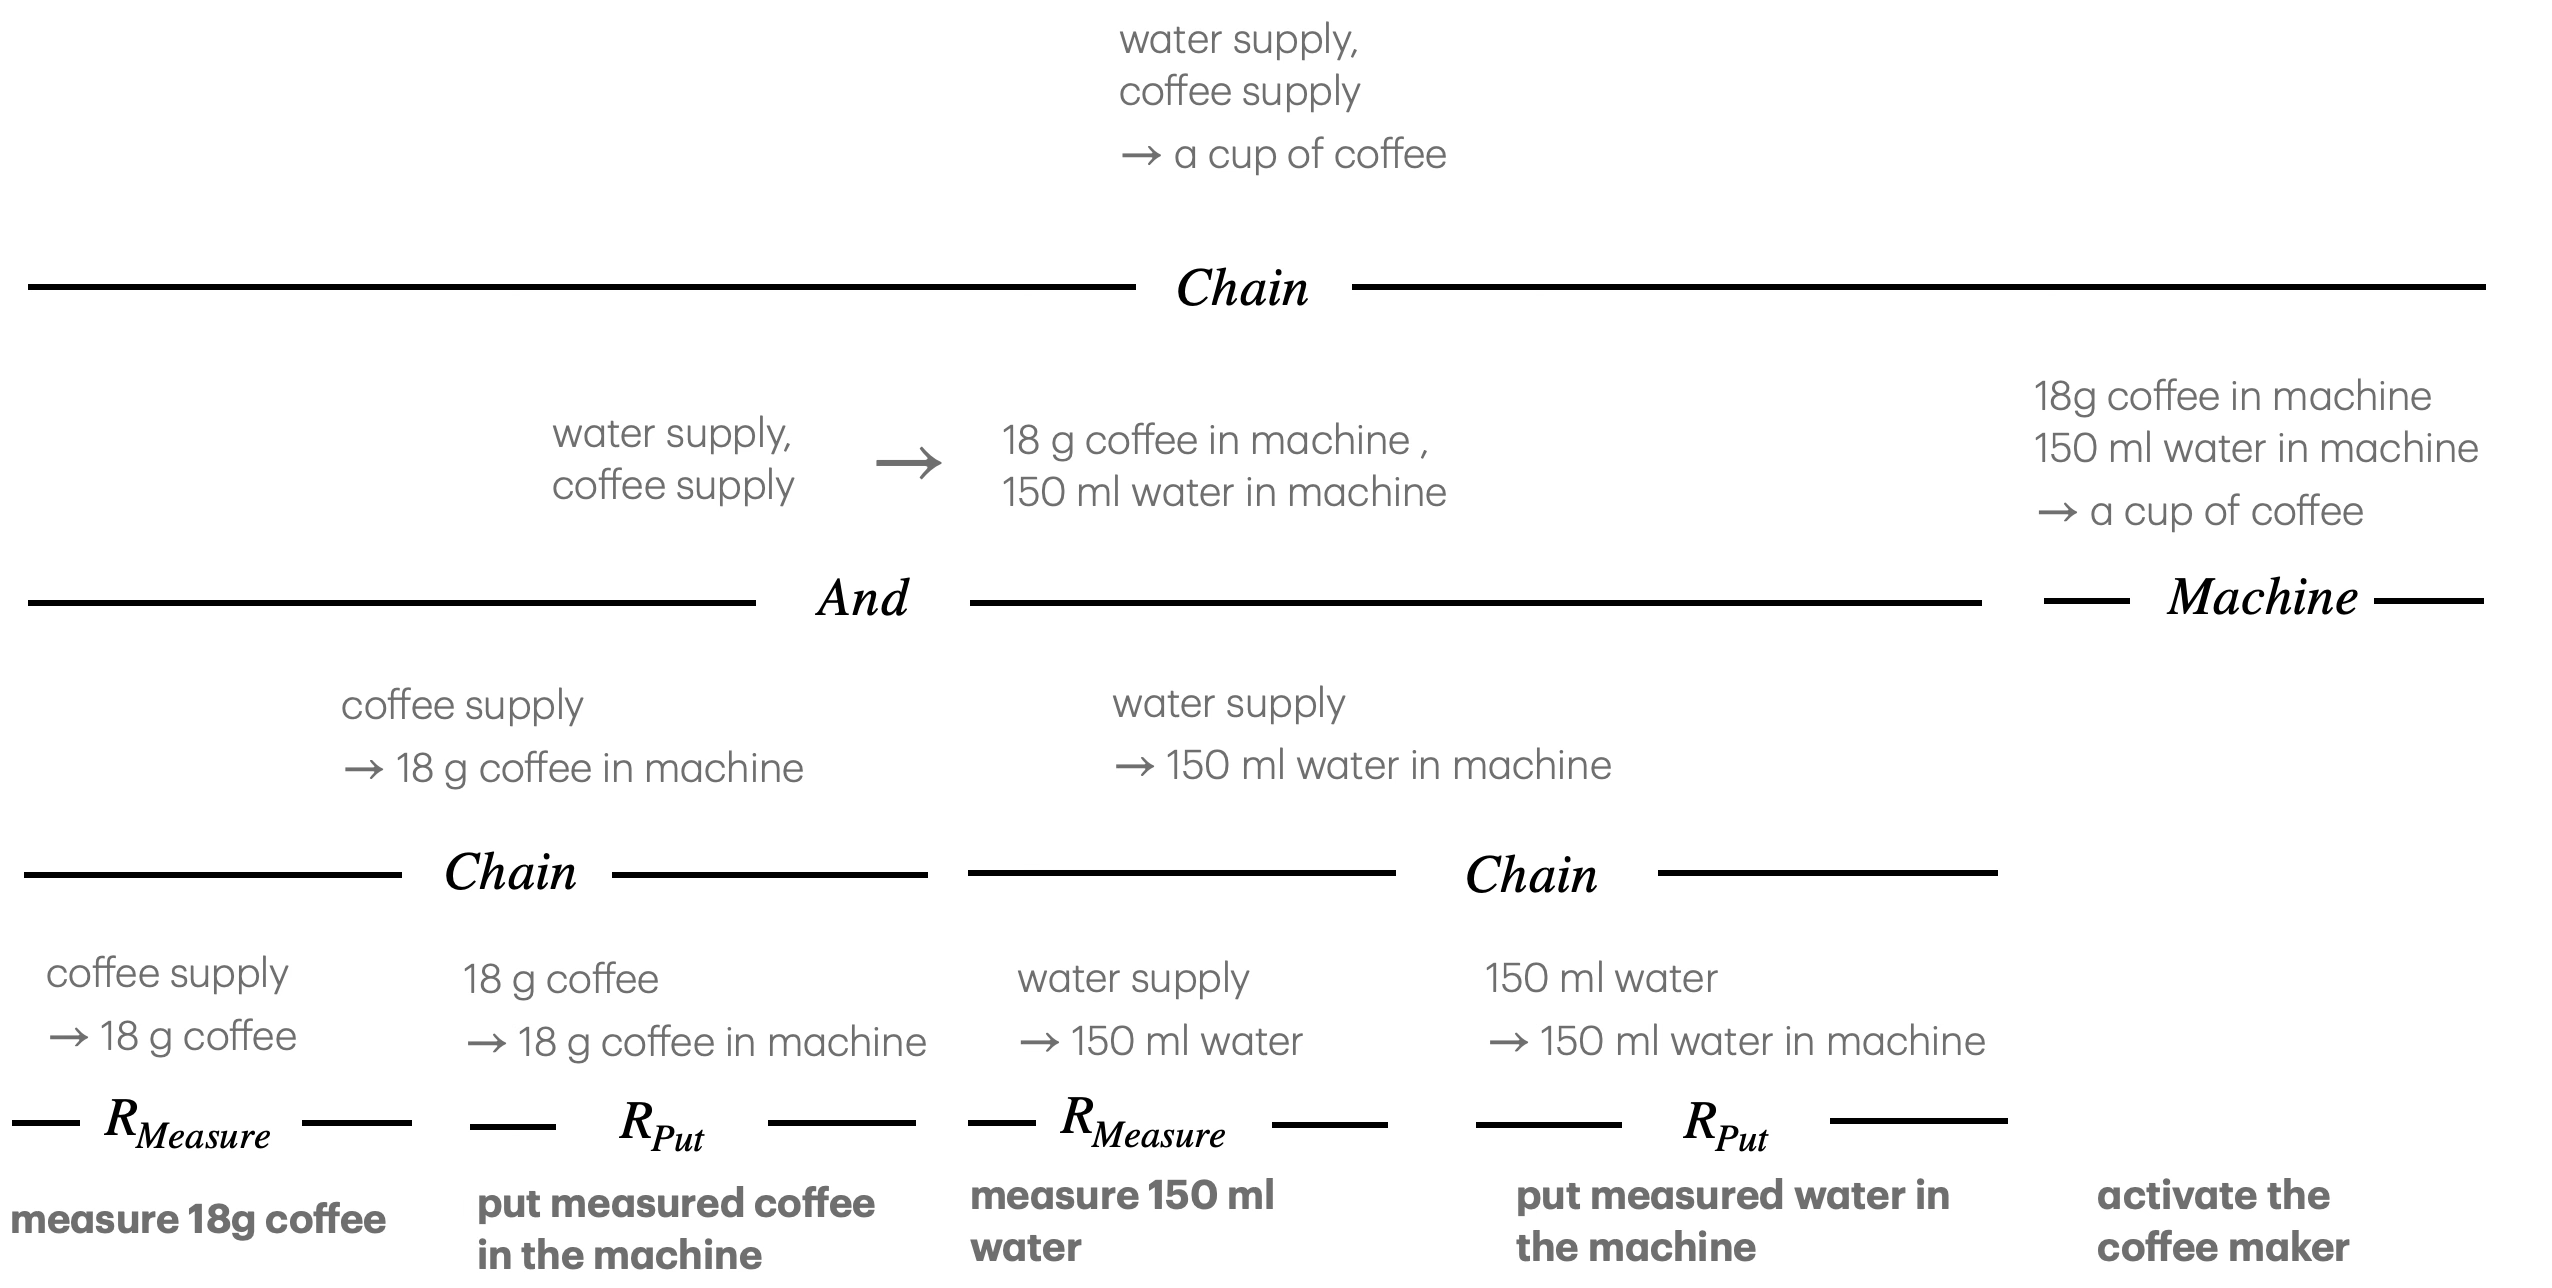
\includegraphics[width=0.9\linewidth]{coffee.png}
%     \caption{}
%     \label{fig: coffee}
% \end{figure}

% \begin{figure}
%     \centering 
%     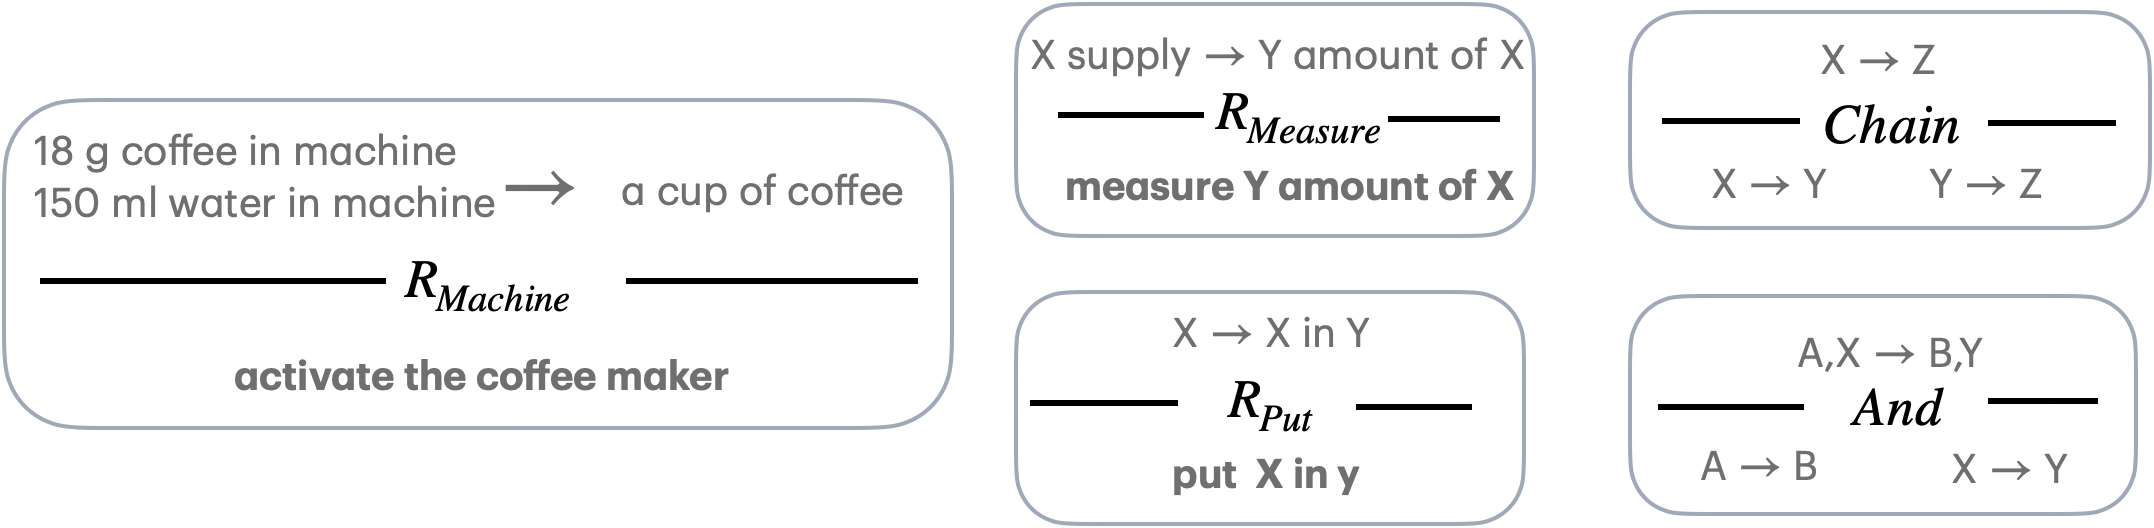
\includegraphics[width=0.9\linewidth]{coffee rule.png}
%     \caption{}
%     \label{fig: coffee rule}
% \end{figure}




